\chapter{Appendix A}
This appendix documents the use of generative AI tools during the completion of this project. AI tools were used in a supporting manner only, mainly for improving clarity and or structure. All technical decisions, implementations, simulations, and interpretations were completed without the use of generative AI.


\section{Example AI prompts used}
The following list provides examples of prompts during the project. Some prompts were excluded when they were substantially similar to others or if they did not contribute to the project. 

\begin{itemize}
    \item Show me this paragraph rewritten in a more formal tone suitable for a thesis
    \item Summarize this section without altering any technical information
    \item Suggest how clarity and structure of this section could be improved 
    \item Suggest a concise caption for this figure (or table etc)
    \item Restructure this section to better show the key points and results 
    \item Show me how the introduction could be rewritten to allow the reader to understand the project objectives better
    \item Revise this methodology description to improve clarity
    \item Improve grammar and sentence structure in this section
    \item Rephrase this explanation
    \item Suggest an improved subsection heading that reflects the existing content
    \item Suggest the structure of this section in terms of headings
    \item Rephrase this explanation to be more concise
\end{itemize}


\section{Code Explanation and Refactoring support}
Aside from LLM inputs on refactoring code or changing comments, no AI was used to generate or create code from scratch. 
\begin{itemize}
    \item Explain this python function in a clearer manner and how it works
    \item Edit the comments to be clearer
    \item Show me how this function could be refactored to improve readability
    \item Reformat this function
    \item Identify areas were the code is ambiguous, with unclear variable names or logical flow and could be made clearer or more readable
    \item Suggest variable names
\end{itemize}


\section{section RA form}
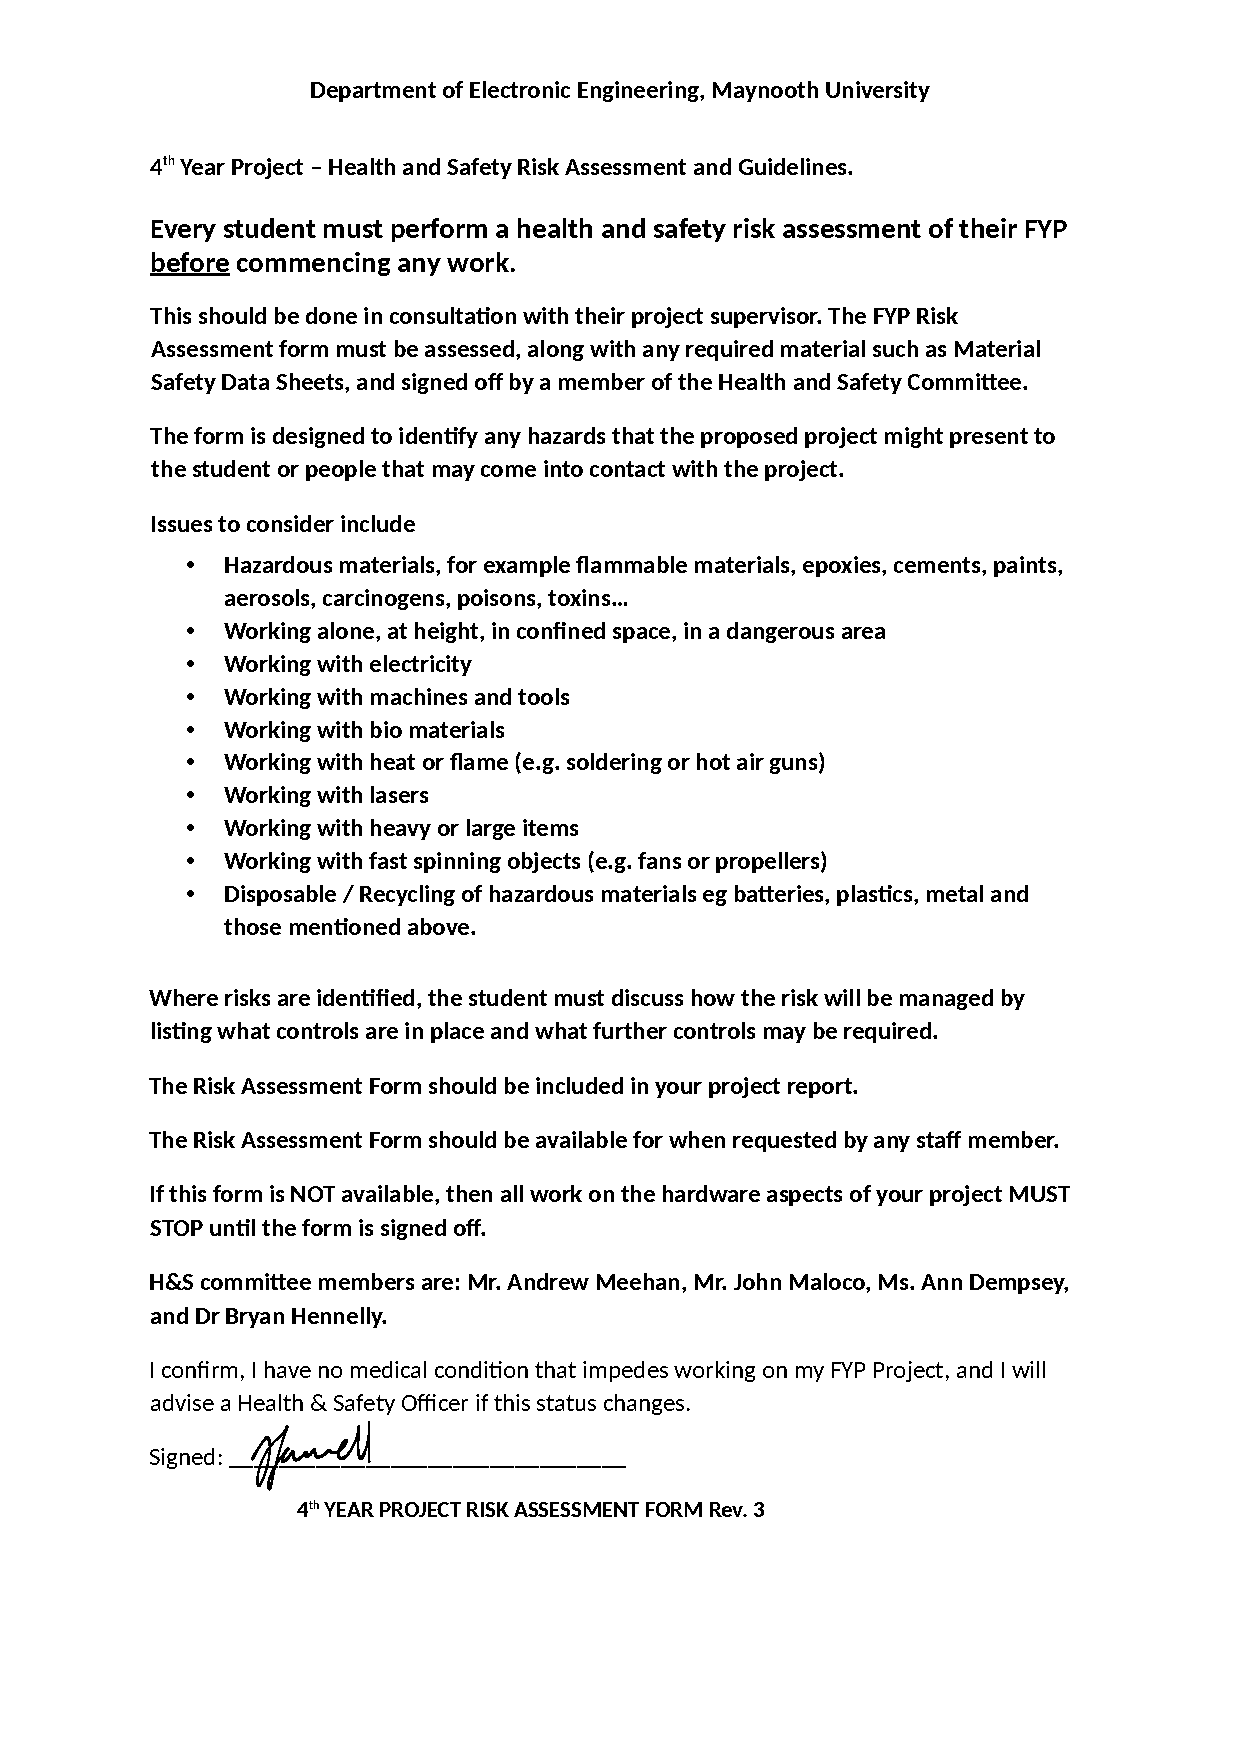
\includepdf[pages=-,scale=0.95]{figures/RaForm.pdf}


\section{GitHub}

All code used to generate results can be found on GitHub \cite{farrell_fyp_2026}. 